%--
\chapter{动态规划 (L19, L20)}


%----------------------------------------
\section*{授课提纲}

\nid 
%--
\begin{itemize}
    \item 
\end{itemize}


\gra

%----------------------------------------
\section{}



%--
\begin{figure}[ht]
    \center
    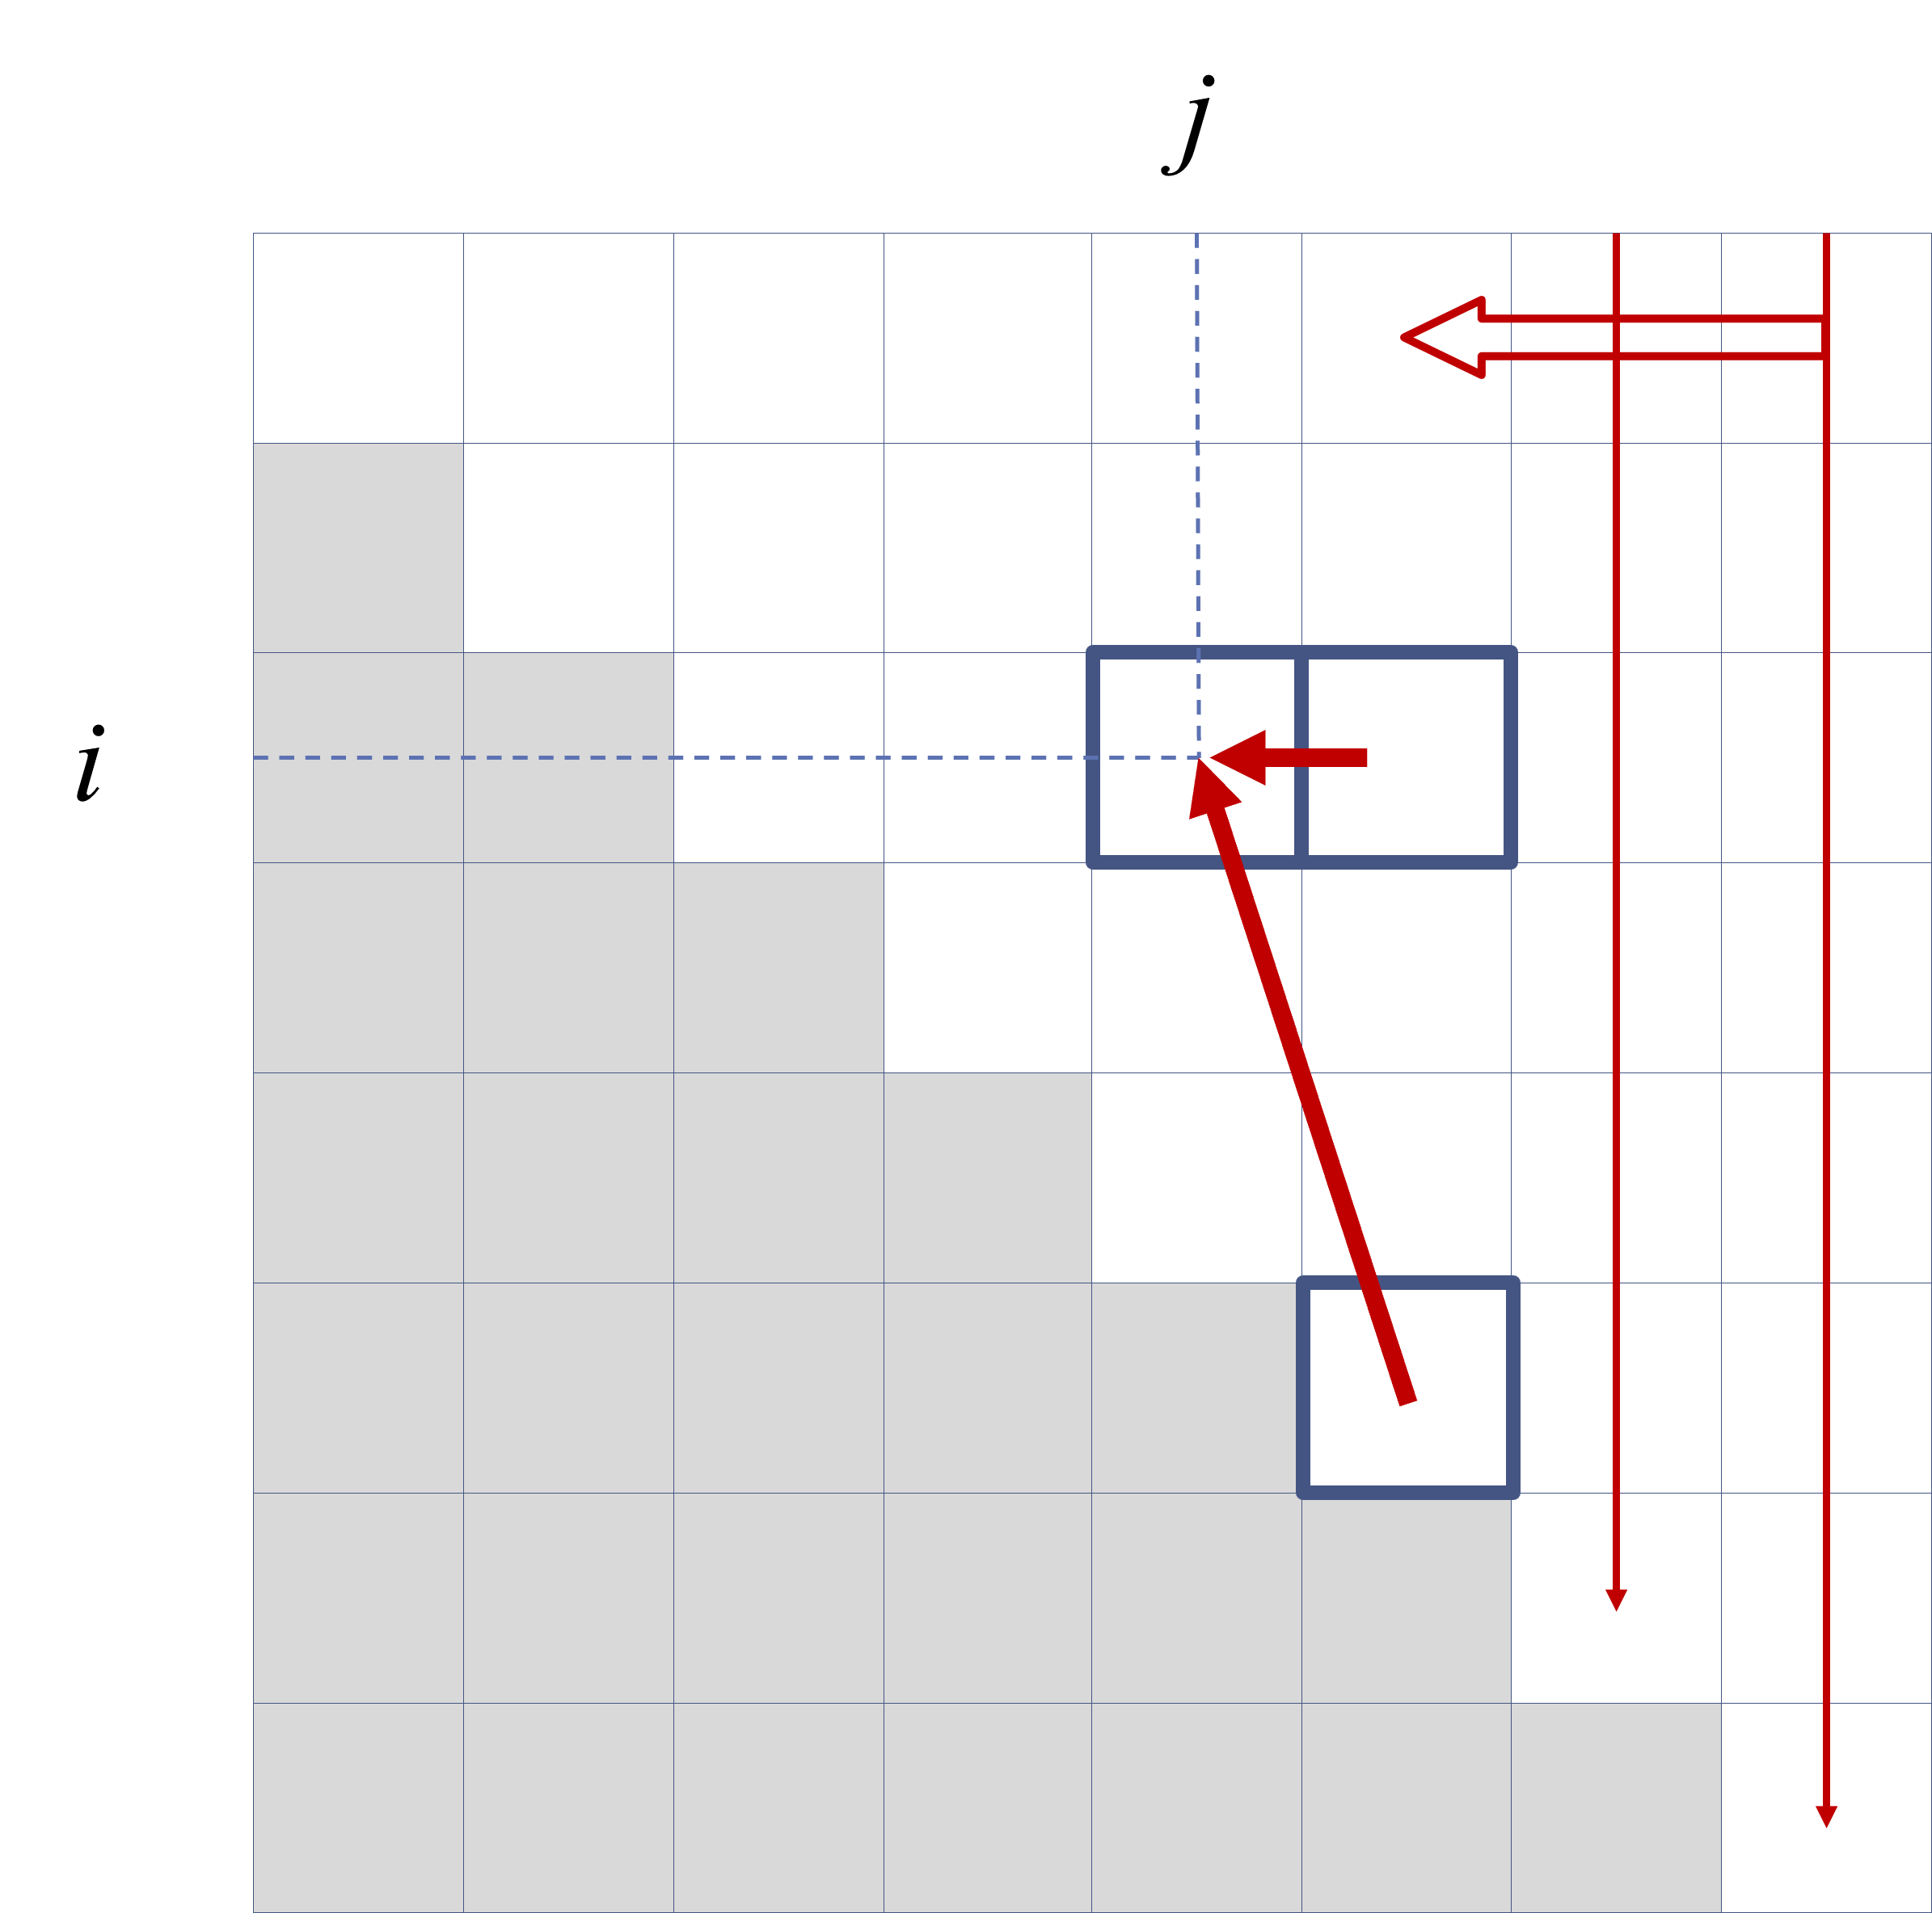
\includegraphics[width=0.5\columnwidth]{./figs/dp/lis.png}
    \caption{子问题依赖关系图}
    \label{fig:lis}
\end{figure}


%--------------------
\subsection{}

%--
\begin{algorithm}[htbp]
    \caption{\alg{LIS-In}($A[1..n]$)}
    \label{}
    \begin{algorithmic}[1]
        \State $A[0] := -\infty$ 
        %
        \For{$i = 0 \textbf{ to } n$}
            \State $L_{in}[i,n+1] := 0$
        \EndFor
        %
        \For{$j = n \textbf{ downto } 1$}
            \For{$i = 0 \textbf{ to } j-1$}
                \If{$A[i] \geq A[j]$}
                    \State $L_{in}[i,j] := L_{in}[i,j+1]$
                \Else
                    \State $L_{in}[i,j] := \max(L_{in}[i,j+1], 1+L_{in}[j,j+1])$
                \EndIf
            \EndFor
        \EndFor
        \State \Return{$L_{in}[0,1]$}
    \end{algorithmic}
\end{algorithm}


%    
%    
%    
%\end{algorithm}


%--------------------
\subsection{}


%--
\begin{algorithm}[htbp]
    \caption{\alg{LIS-Out}($A[1..n]$)}
    \label{}
    \begin{algorithmic}[1]
        \State $A[0] := -\infty$
        %
        \For{$i= n \textbf{ downto } 0$}
            \State $L_{out}[i] := 1$
             \For{$j = i+1 \textbf{ to } n$}
                \If{$\mathrm{(} A[j]>A[i] \mathrm{)}$ and $\mathrm{(} 1+L_{out}[j] > L_{out}[i] \mathrm{)}$}
                    \State $L_{out}[i] := 1+ L_{out}[j]$
                \EndIf
             \EndFor
        \EndFor
        \State \Return{$L_{out}[0] - 1$} 
    \end{algorithmic}
\end{algorithm}


%    
%    
%    
%         \;
%       
%            \If{}{
%                 \;
%            }
%        }
%    }
%    
%    \;
%    
%\end{algorithm}





%%%%%%%%%%%%%%%%%%%%%%%%%%%%%%%%%%%
\iffalse


\nin DP的动机与基本形式：
%--
\begin{itemize}
    \item 朴素递归背后的冗余：以求Fibonacci数为例。
    \item 消除冗余：子问题字典。
    \item 消除依赖：子问题的TO。
\end{itemize}


\nin MIT模板：SRTBOT
%--
\begin{itemize}
    \item \ul{S}ubproblem。
    \item \ul{R}elation。
    \item \ul{T}opo order。
    \item \ul{B}ase case。
    \item \ul{O}riginal problem。
    \item \ul{T}ime、space。
\end{itemize}


\nin DP典型示例：
%--
\begin{itemize}
    \item 矩阵链相乘问题，带权BST问题，Edit distance问题。
    \item LIS问题（\S \ref{Sec:LIS}）。
    \item 高速餐馆问题，文本换行问题。
    \item 换硬币问题。
\end{itemize}

\nin DP视角回顾既有算法：
%--
\begin{itemize}
    \item DAG图上的SSSP。
    \item \alg{Bellman-Ford}。
    \item \alg{Floyd-Warshall}。
\end{itemize}


%--------------------------------------------------------------------------------
\section{LIS问题} \label{Sec:LIS}

给定一个元素序列（sequence），选出其中的若干个元素，并保持这些元素在原始序列中的序不变，则得到该序列的一个子序列（subsequence）。
子序列中的元素不一定是连续的。原序列中截取连续的一段，称为子串（substring）。

假设序列中的元素是两两可比较的，我们要找到一个子序列，其中的元素是严格递增的，这被称为一个递增子序列（increasing subsequence）。

所有递增子序列中，长度最大的即为最长递增子序列（Longest Increase Subsequence，LIS）。

下面我们来讨论如何解决LIS问题。

%----------------------------------------
\subsection{着眼于输入序列}

假设输入序列存放在数组$A[1..n]$中。
无论LIS是什么，其中的元素必然是从$A[1..n]$中选出来的。所以我们的着眼点是输入元素序列$A[1..n]$。
我们只需要对$A[1..n]$中的每个元素问一问，这个元素该不该选，则问题就能解决。

LIS的定义决定了，判定$A[1..n]$中元素是否应该属于LIS这一问题，具有良好的递归结构。
根的定义，subsequence中元素的出现可以是不连续的。所以subsequence可以自然地由更小的 subsequence 拼接而成。

我们这样来看待subsequence问题：当我们选定某个元素$A[i]$时，我们只需递归地求出$A[i+1..n]$中的subsequence，则可以和已经选定的subsequence拼接而成最终要求的subsequence。

在考虑完subsequence的拼接之后，我们来考虑increasing的要求。由于LIS中的元素要求是单调递增的，所以我们求子问题$A[i+1..n]$的LIS时，只能考虑比当前已选元素更大的元素。为此，我们需要将这一要求通过一个参数，传递给新的要求的子问题。
根据上面的分析，我们定义子问题$L_1(i,j)$表示$A[j..n]$中，在所有元素大于$A[i]$的前提下，LIS的长度。
我们设定一个辅助元素$A[0] = -\infty$。我们的目标是计算$L_1(0,1)$。
对所有的$i<j$，我们有：
%--
\begin{align}
    L_1(i,j) = \begin{cases}
        0 & \text{if } j>n \\
        L_1(i,j+1) & \text{if } A[i] \geq A[j] \\
        \max\set{L_1(i,j+1), 1+L_1(j,j+1)} & \text{otherwise}    
    \end{cases} 
\end{align}

上述递归求解的思路非常“蛮力”。它直接考虑子问题的第一个元素$A[j]$的所有可能情况，通过枚举所有可能情况，“硬生生”地将子问题规模缩小了1。

根据递归函数所蕴含的依赖关系，我们只需要以如下的顺序填充数组$L_1[0..n, 1..n+1]$：从右向左，先填满右边一列，再填满左边一列，如图\ref{F:LIS}所示。

%--
\begin{figure}[ht]
    \center
    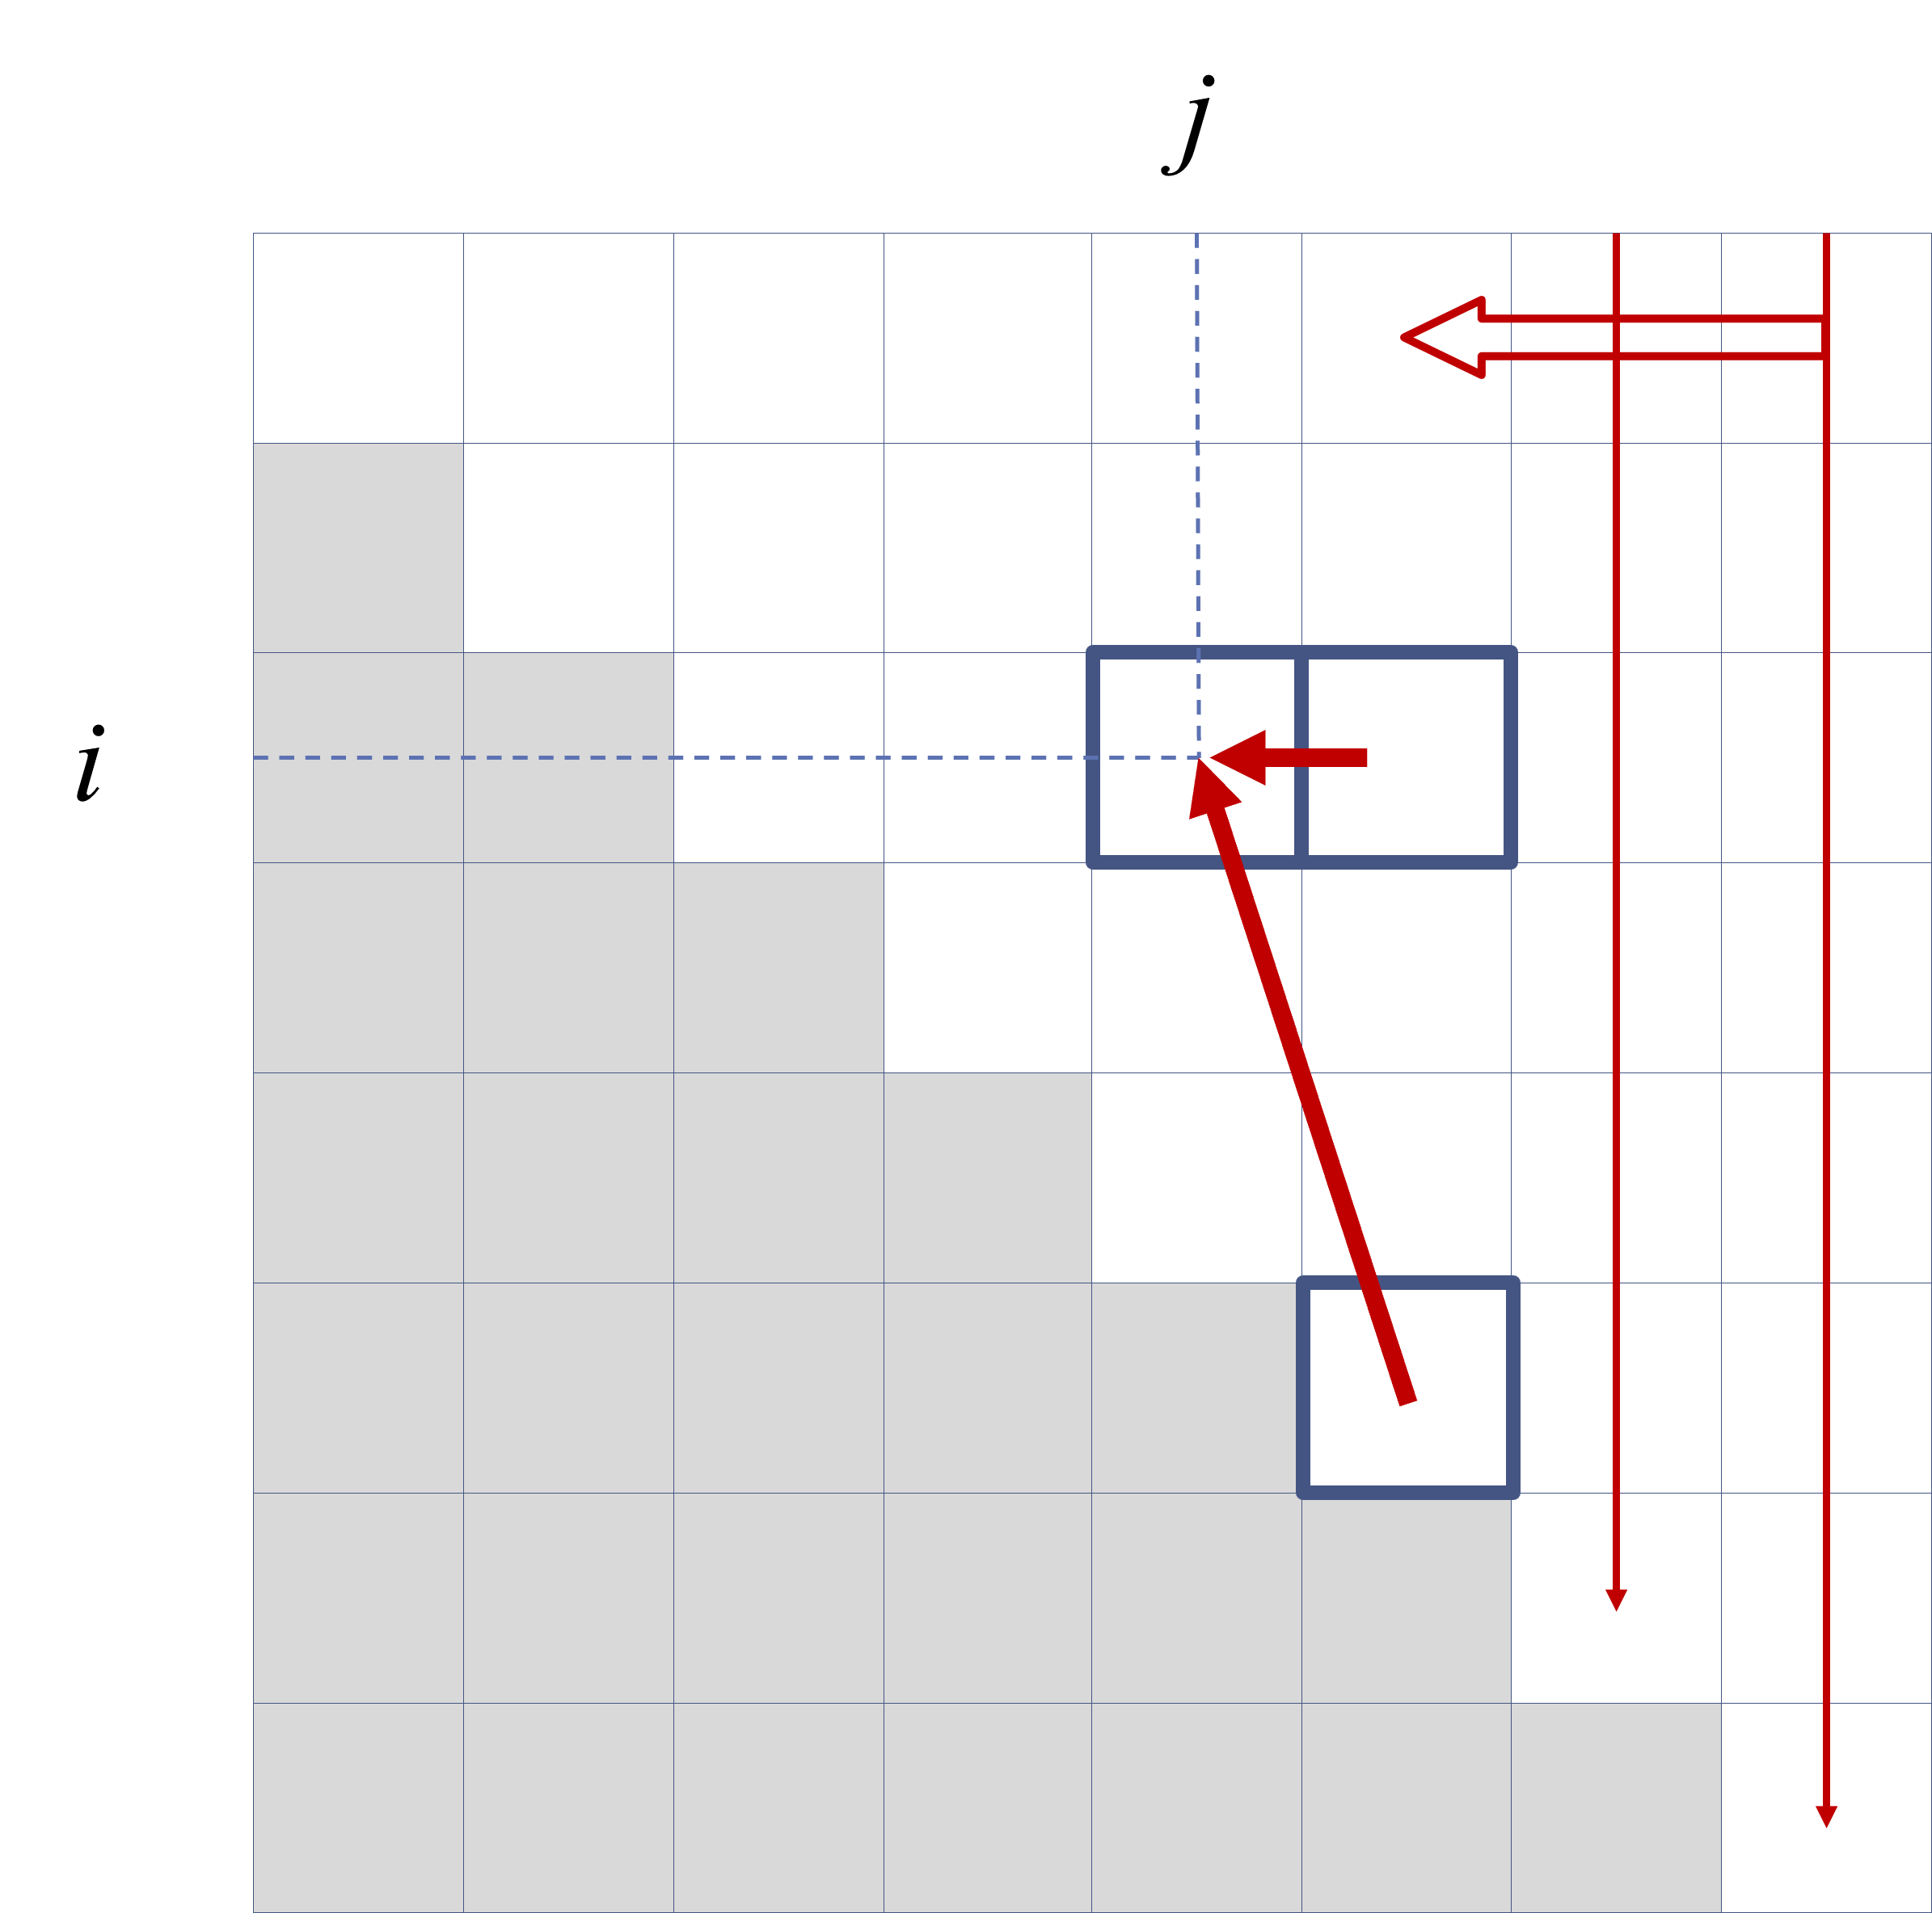
\includegraphics[width=0.35\columnwidth]{./figs/dp/lis.png}
    \caption{子问题依赖关系图}
    \label{F:LIS}
\end{figure}


根据上述递归，我们得出动态规划算法，如算法\ref{A:LIS1}所示。



LIS1算法的时间复杂度为$O(n^2)$，空间复杂度同样为$O(n^2)$。

%--
\begin{algorithm}[ht]
    
    \caption{LIS1($A[1..n]$) \label{A:LIS1} }
    
    $A[0] := -\infty$ \;
    
    \For{$i := 0 \text{ \bf to } n$}{
        $L_1[i,n+1] := 0$ \;
    }
    
    \For{$j := n \text{ \bf downto } 1$}{
        \For{$i := 0 \text{ \bf to } j-1$}{
            \If{$A[i] \geq A[j]$}{
                $L_1[i,j] := L_1[i,j+1]$ \;
            }
            \Else{
                $L_1[i,j] := max \set{L_1[i,j+1], 1+L_1[j,j+1]}$ \;
            }
        }
    }
    
    \Return{$L_1[0,1]$} \;
    
\end{algorithm}



%----------------------------------------
\subsection{着眼于输出序列}

另一种对偶的思路是，我们着眼于考虑输出序列。我们只需要逐个确定LIS中的每个元素，则可以求出LIS。

当我们为LIS选定某个元素$A[i]$时，如果后面有元素$A[j]$大于$A[i]$，则我们潜在地可以通过选择$A[j]$得到更长的递增子序列。
如果我们选定$A[j]$，则问题规模缩小，但是问题不变，我们递归地求解。

对于多个可能的$A[j]$，我们没有更好的办法，还是枚举所有可能，比出最大的。

令$L_2(i)$表示$A[i..n]$中，从$A[i]$开始的LIS的长度，即仅考虑以$A[i]$为第一个元素的subsequence，并从中找出LIS。
我们的目标是计算$L_2[0]-1$。此处减一是为了修正辅助元素$A[0]=-\infty$。
$L_2(i)$满足递归式：
%--
\begin{align}
    L_2(i) = 1 + \max\set{L_2(j) | j>i \text{ and } A[j] > A[i]}
\end{align}

\noindent 此处求$\max$的集合可能为空集，所以我们约定$\max\emptyset = 0$，则$L_2(n) = 1$。

根据递归式，我们发现index小的子问题只会依赖index大的子问题，所以我们按index从大到小的顺序，依次填充一维数组$L_2[0..n]$。

着眼于输出序列，使得我们对于子问题的表示更为精简，所以我们只需要$O(n)$的空间。
但是基于这一更精简的子问题表述，我们需要在所有潜在子问题之间做遍历，所以算法的时间复杂度为$O(n^2)$。

%LIS2算法的空间复杂度为$O(n)$，时间复杂度为$O(n^2)$。

%--
\begin{algorithm}[ht]
    
    \caption{LIS2($A[1..n]$) \label{A:LIS2} }
    
    $A[0] := -\infty$ \;
    
    \For{$i := n \text{ \bf downto } 0$}{
        $L_2[i] := 1$ \;
        \For{$j := i+1 \text{ \bf to } n$}{
            \If{$\mathrm{(} A[j]>A[i] \mathrm{)}$ and $\mathrm{(} 1+L_2[j] > L_2[i] \mathrm{)}$}{
                $L_2[i] := 1+ L_2[j]$ \;
            }
        }
    }
    
    \Return{$L_2[0] - 1$} \;
    
\end{algorithm}

\fi


\bla